\documentclass[12pt]{article}

\setlength{\parindent}{0pt}
\setlength{\parskip}{2mm}

\usepackage{geometry}
 \geometry{
 letterpaper, left=20mm, right=20mm,  top=20mm,
 }
\usepackage{graphicx}
\graphicspath{ {graphics/} }
\usepackage{amssymb}
\usepackage[hidelinks]{hyperref}
\usepackage{wrapfig}
\usepackage[margin=1.2cm]{caption}

%%%%%%%%%%%%%%%%%%% TIKZ CUSTOM SHAPES AND SETTINGS
\usepackage{tikz}
\usetikzlibrary{shapes.geometric, arrows}
\usetikzlibrary{positioning}
\tikzstyle{device} = [rectangle, rounded corners, minimum width=3cm,
	minimum height=1cm,text centered, draw=black] % fill=red!30
\tikzstyle{arrow} = [thick,->,>=stealth]
\tikzstyle{transducer} = [draw,circle,minimum size=1cm,inner sep=0pt]

%%%%%%%%%%%%%%%%%%%%%%%%%%%%%%%%%%%%%%%%%%%%%%%%%
\title{Crab Tracker - Technical Documentation}
%%%%%%%%%%%%%%%%%%%%%%%%%%%%%%%%%%%%%%%%%%%%%%%%%

\author{
	Noah Strong
}

\date{\today\ -- v1.0-wip}

\begin{document}

\maketitle

\tableofcontents{}

\section{Introduction}

The Crab Tracker project was designed as a cost-effective means of remotely
tracking crabs through acoustic signals.
Small piezoelectric transmitters can be waterproofed and attached to crabs,
and their intermittent signals can then be received by a set of four
piezoelectric receivers configured in a square array.

Because this product was built with very few ``off-the-shelf'' components,
it is somewhat complex and many of the finer details may be difficult for
future collaborators to infer based on the existing documentation.
This document aims to provide a technical overview of the project, including
the rationale for some of the design choices, in hopes of giving the reader
a deeper insight into the inner-workings of the product.

\section{Background and Overview}

\subsection{Motivation For The Project}

While solutions already exist to aid in the tracking of aquatic animals,
they are often prohibitively expensive without significant financial resources.
The Crab Tracker product has been designed with cost and simplicity in mind,
so a majority of the components, including both hardware and software, are
custom-made.
However, much of the product, especially the software, has been designed
in a ``modular'' fashion, meaning that the various components are not tightly
coupled.
Simply put, one should be able to change out various components with relative
ease.

\subsection{Description of Components}

Our solution uses high-frequency audio broadcasts to transmit data about
each crab to a central receiving station (likely mounted on a kayak or similar
water vessel).
At the receiving station we have four piezoelectric receivers, or
``hydrophones,'' which are tuned to detect the signals that the crabs'
transmitters broadcast.
These hydrophones are arranged in a square shape with equidistant side
lengths, and all are to be submerged an equal depth into the water.

As acoustic transmissions reach the hydrophone receivers, two distinct
processes must be run.
The first process is to detect incoming signals and label them with accurate
timestamp values.
Once this is done, software must run calculations using these timestamps
to decode the unique identifiers of the broadcasting transmitter(s) and to
determine the direction from which the sound(s) originated.
Because the later task requires a number of calculations, and therefore
processing time,
and because the former task requires low-latency monitoring of the input
devices, each task must be performed on a separate physical computer.

The first device in the chain, whose task is to timestamp incoming data,
need only be a simple microcontroller.
For our purposes, we have tested the system with an Arduino Nano, a small,
inexpensive device with a clock speed of 16MHz.
Once broadcasts are detected and labeled with a timestamp, the device can
send this data to the main computer that will run the calculations.
We originally investigated using the popular I$^2$C protocol for this, but
unfortunately I$^2$C can't be interrupted during a transfer, and therefore
the device would be effectively frozen (and therefore unable to detect
incoming data) any time a transfer was in progress.
If any data were to come into the device during a transfer, its timestamp
would be delayed and therefore inaccurate.
Instead, we opted to use a similar protocol, Serial Perhipheral Interface
(SPI).
The advantage of SPI is that data can be placed into a separate physical
bus on the device when it is ready, and the other machine can pull data out
of that bus without affecting the detection and timestamp code.

The second device, which runs calculations and displays results to the user,
is a slightly more powerful machine.
We opted to use a Raspberry Pi Model 3B for this task, as these machines are
inexpensive, reasonably powerful, SPI-compatible, and more.
We also purchased a 7-inch touchscreen for use in the field.
The Pi is directly wired to the Arduino for SPI.
See Figure \ref{fig:component-diagram} for an illustration of these components.

\begin{figure}[h]
\begin{center}
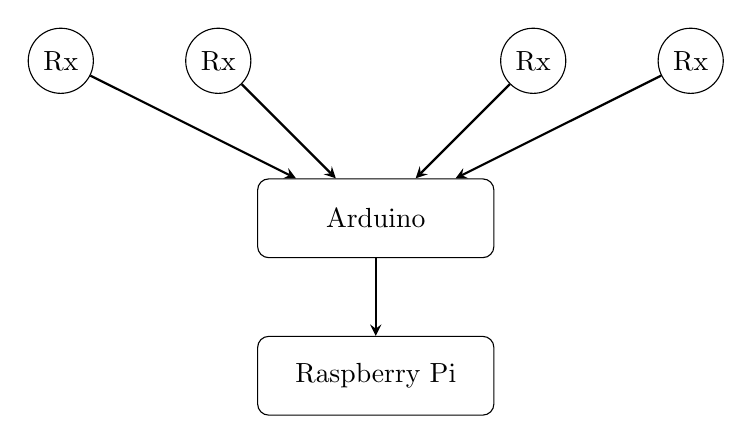
\begin{tikzpicture}[node distance=2cm]
%\node (tx) [draw=none, circle]                 {};
%\draw (tx) circle (0.9);
%\draw (tx) circle (1.3);

%--------- Receivers ---------%
%\node (rx1) [draw, circle, below of = tx]  {Rx};
\node (rx1) [draw, circle               ]  {Rx};
\node (rx2) [draw, circle, right of = rx1] {Rx};
\node (CTR) [rectangle, draw=none, right of = rx2] {};
\node (rx3) [draw, circle, right of = CTR] {Rx};
\node (rx4) [draw, circle, right of = rx3] {Rx};

%--------- Devices ---------%
\node (arduino) [device, below of = CTR] {Arduino};
\node (pi) [device, below of = arduino] {Raspberry Pi};

%--------- Arrows ---------%
\draw [arrow] (rx1) -- (arduino);
\draw [arrow] (rx2) -- (arduino);
\draw [arrow] (rx3) -- (arduino);
\draw [arrow] (rx4) -- (arduino);
\draw [arrow] (arduino) -- (pi);

\end{tikzpicture}
\end{center}
\caption{A simple diagram detailing the main components.}
\label{fig:component-diagram}
\end{figure}

While both the Arduino and the Raspberry Pi were off-the-shelf products,
the transmitter and receiver hardware was all custom designed and fabricated
for use in this project.
Clearer specifications, including detailed diagrams, are detailed in other
documents and therefore many details will not be repeated here.

\section{Electronics Hardware}\label{sec:ee-hardware}

\subsection{Transmitters}

The transmitters are small piezoelectric transducers that oscilate at an
ultrasonic frequency.
In our work, this frequency has been in the 40-60kHz range, depending on the
resonant frequency of the transducer itself.
Though we have not established bounds on our range of potential frequencies,
the actual frequency shouldn't matter so long as the receiving hardware is
appropriately tuned to pick up this frequency (through filtering, hardware,
etc.).

Each transmitter is attached to a small printed circuit board designed
specifically for the project.
The PCB can power the transducer by feeding it a current, effectively turning
it off or on as needed.
Each board will be programmed with a unique identifier (a numeric value).
The ID determines the patter of pulses that the transmitter should emit.
For more details on this, see the iCRAB Transmission Protocol document.

\subsection{Receivers}

The receivers include small piezeoelectric transducers that are able to detect
vibrations in the same range as the transmitters.
A preamplifier steps up the signal from the transducer before sending this
signal along to a bandpass filter.
The bandpass filter restricts the frequencies that the hardware ``listens''
to, meaning that a lot of irrelevant noise can be discarded.
After being filtered, the signal is then amplified again before being
rectified (effectively producing the absolute value of the incoming sine wave).
The low pass filter does ???
Finally, the Schmitt Trigger acts as a variable threshold, preventing the
rising or falling edge from being interpreted as a series of short rising and
falling edges.
Finally, the resul resulting digital signal is sent over a wire to the timestamp
recorder which is detailed in section \ref{sec:ts-rec}.
See Figure \ref{fig:rx-detail} for details on this pipeline.

\begin{figure}[h]
\begin{center}
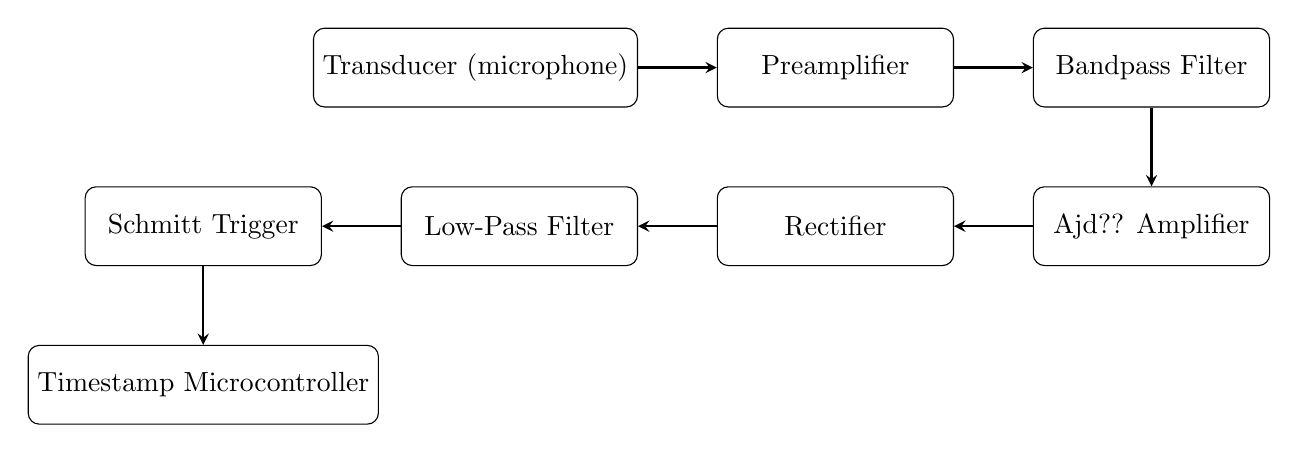
\begin{tikzpicture}[node distance=1cm]

\node (mic)    [device]                    {Transducer (microphone)};
\node (preamp) [device, right = of mic]    {Preamplifier};
\node (bp)     [device, right = of preamp] {Bandpass Filter};

\node (adjamp) [device, below = of bp]    {Ajd?? Amplifier};
\node (rect)   [device, left = of adjamp] {Rectifier};
\node (lowp)   [device, left = of rect]   {Low-Pass Filter};
\node (schmt)  [device, left = of lowp]   {Schmitt Trigger};

\node (ard)    [device, below = of schmt] {Timestamp Microcontroller};

\draw [arrow] (mic) -- (preamp);
\draw [arrow] (preamp) -- (bp);
\draw [arrow] (bp) -- (adjamp);
\draw [arrow] (adjamp) -- (rect);
\draw [arrow] (rect) -- (lowp);
\draw [arrow] (lowp) -- (schmt);
\draw [arrow] (schmt) -- (ard);

\end{tikzpicture}
\end{center}
\caption{The receiver hardware pipeline.}
\label{fig:rx-detail}
\end{figure}

\section{Computer Hardware}\label{sec:cs-hardware}

\subsection{Timestamp Recorder}\label{sec:ts-rec}

\section{Software}\label{sec:software}

\end{document}

